%!TEX root = Physics231.tex

\chapter{Green's Functions}
\label{ch:P231:summary}

We summarize the bits of the earlier chapters relevant for our study of Green's functions. \flip{To do: merge this in more cleanly.}

\section{The Green's Function Problem}

The Green's function can be defined by analogy to the finite-dimensional inverse transformation. The finite-dimensional linear system $A\vec v = \vec w$ can be solved by applying the inverse transformation $A^{-1}$ in the same way that the continuum (infinite-dimensional) system $\mathcal O \psi(x) = s(x)$ can be solved with the Green's function $G(x,y)$ of the operator $\mathcal O$:
\begin{align}
  v^i &= \sum_i 
  \mat{\left(A^{-1}\right)}{i}{j} w^j
  &\Rightarrow
  &
  &
  \psi(x) &= \int  \D{y}\, G(x,y)\, s(y) \ .
  \label{eq:def:of:function:space:Greens:function}
\end{align}
We explicitly write the sum over the dummy index $i$ to emphasize the analogy to the integration over the dummy variable $y$. The arguments of the functions play the role of `continuum indices.'

\section{Differential Operators}

Linear transformations on function space are differential operators. In principle you can imagine linear transformations that are not differential operators, for example a finite translation. However, because our models of nature are typically \emph{local} and \emph{causal}, the linear transformations that we obtain from physical models are differential operators\footnote{This is not to say that finite transformations are somehow not permitted. The dynamics that govern our models of nature, however, only dictate how information is transmitted infinitesimally in space and time. Propagation forward in time by some finite interval is described by the exponentiation of infinitesimal forward time translations. This is, of course, why the time-translation operator in quantum mechanics is $e^{i\hat H t}$, where the Hamiltonian $H$ is described as a local function with perhaps one or two derivative operators.}. 

Let's write a general differential operator as:
\begin{align}
  \mathcal O = 
  p_0(x) 
  + p_1(x) \frac{d}{dx}
  + p_2(x) \left(\frac{d}{dx}\right)^2
  + \cdots
  \label{eq:summary:differential:operator}
\end{align}
where the $p_i(x)$ are polynomials. Sometimes we will write this as $\mathcal O_x$ to make it clear that the argument of the polynomials is $x$ and the variable with which we are differentiating is $x$.  
\begin{exercise}
Explain why \eqref{eq:summary:differential:operator} is a linear operator acting on function spaces.
\end{exercise}
\begin{exercise}
A confused colleague argues to you that \eqref{eq:summary:differential:operator} cannot possibly be `linear.' Just look at it, your colleague says: the functions $p_i(x)$ are polynomials---those aren't \emph{linear}! There are also powers of derivatives---how is that possibly linear? Explain to your colleague why the $p_i(x)$ does not have to be linear nor is one restricted to finite powers of derivatives for the operator $\mathcal O$ to be a linear operator acting on function space.
\end{exercise}
Technically \eqref{eq:summary:differential:operator} is called a \textbf{formal operator} because we haven't specified the boundary conditions of the function space. Recall in our discretized `histogram space' in Section~\ref{sec:histogramspace} that we had to be careful about how to define the derivative acting on the boundaries of the space. A differential operator along with boundary conditions is called a \textbf{concrete operator}.

\section{Inner Product}

There's a convenient inner product that you may be familiar with from quantum mechanics. For two functions $f(x)$ and $g(x)$ in your function space, define the inner product to be
\begin{align}
  \langle f,g\rangle 
  =
  \int \D{x}\, f^*(x)g(x) \ .
  \label{eq:summary:L2:inner:product}
\end{align}
\begin{example}
Wave functions in 1D quantum mechanics obey this norm. For an infinite domain, we typically restrict to square-integrable functions meaning that $|f|^2$ goes to zero fast enough at $\pm \infty$ so that the integral $\langle f, f\rangle$ is finite. 
\end{example}
Sometimes the inner product is defined with respect to a \textbf{weight} function $w(x)$:
\begin{align}
  \langle f,g\rangle_w 
  =
  \int \D{x}\, w(x)\, f^*(x)g(x) \ .
  \label{eq:summary:weighted:inner:product}
\end{align}
There's nothing mysterious about inner products with weights. They typically boil down to the fact that one is not using Cartesian coordinates. 
\begin{example}
Have you met the Bessel functions? If not, you're in for a treat in your electrodynamics course. The Bessel functions satisfy a funny orthogonality relation with weight $w(x)\sim x$ because they show up as the radial part of a solution when using polar coordinates. When you separate variables, $d^2x = r\D{r}\,\D{\theta}$, we see that the measure over the radial coordinate $r$ carries a \emph{weight} $r$.
\end{example}
We will assume unit weight until we go to higher spatial dimensions\sidenote{My dissertation focused on theories of extra dimensions. I also noticed that my weight increased in my final year of graduate school as I spent most of my time writing about extra dimensions and eating cafe pastries.}.


\section{Dual Vectors}

What are the `dual functions' (dual vectors, bras) in function space? These are linear functions on act on functions and spit out numbers. These are integrals that are pre-loaded with some factors. Assuming unit weight:
\begin{align}
  \langle f | = \langle f, \qquad \rangle
  = 
  \int \D{x} \, f^*(x) \left[\text{ insert ket here }\right] \ .
\end{align}




\section{Adjoint operators}

What is the adjoint of a differential operator? The definition of the adjoint \eqref{eq:def:adjoint} and the function space inner product \eqref{eq:summary:L2:inner:product} give us a hint. We define $\mathcal O^\dag$ by the property
\begin{align}
  % \int \D{x} \, \left[\mathcal O f(x)\right]^* g(x)
  % = 
  % \int \D{x} \, f^*(x) \left[\mathcal O^\dag g(x)\right] \ .
  \int \D{x} \, f(x)^* \left[\mathcal O g(x)\right]
  \equiv
  \int \D{x} \, \left[\mathcal O^\dag f(x)\right]^*  g(x) \ .
\end{align}
The strategy is: given an inner product (integral) over $f^*$ and $g$ where there is some stuff ($\mathcal O$) acting on $g$, can we re-write this as an integral with no stuff acting on $g$ and some \emph{other} stuff acting on $f^*$? If so, then the `other stuff' is the adjoint $\mathcal O^\dag$.
\begin{example}
What is the adjoint of the derivative operator, $\mathcal O = \D{}/\D{x}$? Assume an interval $x\in[a,b]$ and Dirichlet boundary conditions, $f(a)=f(b)=0$. There's a simple way to do this: integrate by parts.
\begin{align}
  \int \D{x} \,  f(x) \left[\frac{d}{dx} g(x)\right]
  &=
  - \int \D{x} \, \left[\frac{d}{dx}f(x)\right]^* g(x)
  +
  \left[f^*(x)g(x)\right]^b_a \ 
  \\
  &= \phantom{+}
  \int \D{x} \, \left[-\frac{d}{dx}f(x)\right]^* g(x)
  \ . 
\end{align}
From this we deduce that
\begin{align}
  \left(\frac{\D{}}{\D{x}}\right)^\dag = - \frac{\D{}}{\D{x}} \ .
\end{align}
\end{example}

We are especially interested in \textbf{self-adjoint} (Hermitian) operators for which
\begin{align}
  \mathcal O^\dag = \mathcal O \ .
\end{align}
This is, as we mentioned for the finite-dimensional case, because self-adjoint operators are \emph{nice}: they have real eigenvalues and orthogonal eigenvectors. Since most physical values are real eigenvalues of some operator, one may expect that the differential operators that show up in physics are typically self-adjoint.
\begin{exercise}
We saw above that the derivative operator is not self-adjoint. What is an appropriate self-adjoint version of the derivative operator? \emph{Hint: what is the momentum operator in quantum mechanics?}\footnote{\url{https://aapt.scitation.org/doi/abs/10.1119/1.9932}} 
\end{exercise}
\begin{example}
Consider $\mathcal O = -\partial_x^2$ defined on the domain $x\in [0,1]$ with the boundary conditions $f(0)=f(1)=0$. Is this operator self-adjoint? We want to check of $\langle f,\mathcal O g\rangle = \langle O f, g \rangle$. We have one trick: integration by parts. Let's see how this works.
\begin{align}
  \langle f, \mathcal O g\rangle &= - \int dx\, f^*(x)\partial^2 g(x) \ .
\end{align}
This is compared to
\begin{align}
  \langle \mathcal O f, g\rangle 
  &= -\int^1_0 \D{x }\, \left[\partial^2 f(x)\right]*g(x) 
  \\
  &= 
  -\left.\left(\partial f(x)\right)^*g(x)\right|^1_0
  + \int^1_0 \D{x} \, \left[\partial f(x)\right]^* \partial g(x) 
  \\
  &= \left.f^*(x)\partial^2 g(x)\right|^1_0
  - \int^1_0 \D{x} \, f^*(x) \partial^2 g(x)  
  \\
  &=
  - \int^1_0 \D{x} \, f^*(x) \partial^2 g(x)  
  \ .
\end{align}
And so we see that indeed $(-\partial^2)^\dag = -\partial^2$.
\end{example}
\begin{exercise}
In the previous example, what is the significance of the overall sign of the operator? \emph{Hint: the sign doesn't matter, it's because we typically think of $-\partial^2$ and its higher-dimensional derivatives as the square of the momentum operator.}
\end{exercise}
\begin{example}\label{ex:summary:eigenfunction:fourier}
The \textbf{eigenfunctions} $f_n$ of $-\partial^2$ defined on $x\in [0,1]$ with Dirichlet boundary conditions are simply 
\begin{align}
  f_n(x) &= A_n \sin(n\pi x) 
  &
  \lambda_n = - n^2\pi^2 \ ,
  \label{eq:summary:fourier:basis:unit:interval}
\end{align}
where $\lambda_n$ is the associated eigenvalue and $A_n$ is some normalization that. These eigenfunctions are orthonormal in the following sense:
\begin{align}
  \langle f_n, f_m\rangle = \int_0^1 \D{x} \, \sin(n\pi x)\sin(m\pi x) = \frac{A_nA_m}{2} \delta_{nm} \ ,
\end{align}
from which we deduce that the normalization is $A_n = \sqrt{2}$. That's basically all there is to know about Fourier series.
\end{example}
\begin{exercise}
What would change if we had instead assumed Neumann boundary conditions? What if we had assumed periodic boundary conditions? What about anti-periodic boundary conditions?
\end{exercise}
\begin{exercise}\label{ex:summary:eigenfunction:fourier:2}
A function $g(x)$ defined on an interval $x\in [0,1]$ with Dirichlet boundary conditions can be written with respect to the Fourier basis \eqref{eq:summary:fourier:basis:unit:interval}. In ket notation, the $n^\text{th}$ component of $g$ with respect to this basis is
\begin{align}
  g^n = \langle f_n| g\rangle \ .
\end{align}
Confirm that this is precisely what you know from Fourier series. In other words, we can decompose $g(x)$ as
\begin{align}
  g(x) &= \sum_n \langle f_n| g\rangle f_n(x)  \ .
\end{align}
\end{exercise}

\section{Completeness in Function Space}

We rarely have much to say about the unit matrix in linear algebra. However, much like when we discussed units, we can squeeze a lot out of inserting the identity in our mathematical machinations. In order to help with translate this to function space, let's review how it works in finite dimensional vector spaces. The unit matrix is $\mathbbm{1}$ and may be written:
\begin{align}
  \mathbbm{1} = \sum_i |i\rangle\langle i| \ ,
  \label{eq:unit:matrix}
\end{align}
where $|i\rangle$ and $\langle j|$ are basis (dual-)vectors. 
\begin{exercise}
Take a moment and convince yourself that \eqref{eq:unit:matrix} is true and obvious. It may be helpful to explicitly write out $|i\rangle \langle j|$ as a matrix. 
\end{exercise}
\begin{exercise}\label{ex:completeness:for:non:cartesian:basis}
Suppose you have a two-dimensional Euclidean vector space. Show that \eqref{eq:unit:matrix} is true for the basis
\begin{align}
  |1 \rangle &= 
  \frac{1}{\sqrt{2}}
  \begin{pmatrix}
  1 \\ 1
  \end{pmatrix}
  &
  |2 \rangle &= 
  \frac{1}{\sqrt{2}}
  \begin{pmatrix}
  1 \\ -1
  \end{pmatrix}
  \\
  \langle 1 | &= 
  \frac{1}{\sqrt{2}}
  \begin{pmatrix}
  1 & 1
  \end{pmatrix}
  &
  \langle 2 | &= 
  \frac{1}{\sqrt{2}}
  \begin{pmatrix}
  1 & -1
  \end{pmatrix} \ .
\end{align}
\end{exercise}
In fact, \eqref{eq:unit:matrix} defines what it means that a set of basis vectors is \textbf{complete}. You can write any vector $|v\rangle$ with respect to the basis $|i\rangle$---the components are simply
\begin{align}
  v^i = \langle i | v \rangle
\end{align}
so that 
\begin{align}
  |v\rangle = \sum_i |i\rangle \langle i | v \rangle \ ,
  \label{eq:summary:completeness:by:inserting:1}
\end{align}
which we recognize as nothing more than `multiplying by the identity.' 
%

What does completeness look like in function space?
% 
Let $e_{n}(x)$ be a set of basis functions. The basis is \textbf{complete} if
\begin{align}
  \sum_n \left[e_{n}(x)\right]^* e_{n}(y) = \delta(x-y) \ .
  \label{eq:summary:function:space:completeness}
\end{align}


Compare this \emph{very carefully} with the completeness relation \eqref{eq:unit:matrix}. The sum over $i$ in the finite-dimensional case has been relabeled into a sum over $n$ in the function space---this is just my preference\footnote{I think this is because we will deal with complex functions and I want to avoid using $i$ as an index. But if we're being honest, it's just become a habit.}. The $\mathbbm{1}$ has been replaced by a Dirac $\delta$-function, $\delta(x-y)$. Let's confirm that this makes sense. The \emph{multiply by one} completeness relation \eqref{eq:summary:completeness:by:inserting:1} in function space is
\begin{align}
  |g\rangle 
  &= 
  \sum_n |e_{n}\rangle\langle e_{n}| g\rangle
  &
  \langle e_{n}| g\rangle &=
  \int \D{y} \, [e_{n}(y)]^* g(y) \ .
\end{align}
We have deliberately changed the name of the integration variable to $y$ to avoid confusion; since this variable is integrated over it's simply a \emph{dummy variable} and it doesn't matter what we name it---the quantity $\langle e_{n}|g\rangle$ is independent of $y$ because $y$ is integrated over\footnote{By the way, this should ring a bell from our summation convention. When an upper and lower tensor index are contracted, the resulting object behaves as if it didn't have those indices: $\mat{A}{i}{j}v^j$ behaves as a vector with one upper index.}. Writing this out explicitly as functions:
\begin{align}
  g(x) &= \sum_n\left[\int \D{y}\, e_{n}^*(y)g(y)\right] e_{n}(x) \ .
  \label{eq:summary:complenesss:function:space:in:action}
\end{align}
The factor in the square brackets is simply $\langle e_{n}| g\rangle$, which is just a \emph{number}---it has no functional dependence on $x$.
If this seems unusual, please refer back to Example~\ref{ex:summary:eigenfunction:fourier} and Exercise~\ref{exe:eigenfunction:fourier}. 

By the way, you'll often hear people (perhaps even me) say that the Dirac $\delta$ function is not strictly an \emph{function} but rather a \textbf{distribution}---this means that it only makes sense when it is integrated over. As physicists we'll sometimes be sloppy and talk about physical quantities that could be Dirac $\delta$-functions. There is \emph{never} an appropriate, measurable physical quantity that is described by a $\delta(x)$. Anything with a $\delta(x)$ is an object that was meant to be integrated over. When you imagine that a point charge density is a $\delta$-function, this is only because you will eventually integrate over it to determine the total charge. 
% This is precisely what we saw in the charged cat in Example~\ref{eq:charged:cat}. 
If you ever calculate a \emph{measurable} quantity to be $\delta(x)$ check your work. If you ever find $\delta(x)^2$, then go home, it's past your bed time.

\begin{example}
One can vaguely motivate the $\delta$-function as the unit matrix by appealing to the `histogram basis' of discretized function space. In an ordinary finite-dimensional vector space, unit matrix can be written as
\begin{align}
  \mathbbm{1} = |1\rangle\langle 1 | + |2\rangle\langle 2 | + \cdots
  = \sum_{i,j}\delta_{i}^j|i\rangle\langle j| \ .
\end{align}
The Dirac $\delta$-function in histogram space is analogous to
\begin{align}
  \delta(x-x') &\to \delta_{x}^{x'}|x\rangle\langle x'| \ ,
\end{align}
where $x$ and $x'$ are discrete bins on the right-hand side. Thus for a discretized function $f = f(x_1)|x_1\rangle + f(x_2)|x_2\rangle + \cdots$, one has
\begin{align}
  \int \D{y}\, \delta(x-y) f(y) = f(x) \longrightarrow \sum_j \delta_{x_j}^{x_i}|x_i\rangle\langle x_j| f\rangle  =  f(x_i) |x_i\rangle\ .
\end{align}
\end{example}

\section{Orthonormality in Function Space}

One should contrast the notion of completeness of a a basis this with that of \textbf{orthonormality} of the basis. Orthonormality is the statement that
\begin{align}
  \langle i | j \rangle = \delta^j_i \ .
\end{align}
Completeness has to do with the `outer product' $|i\rangle \langle i|$ while orthonormality has to do with the `inner product' $\langle i | i\rangle = \langle i, i\rangle$. The function space generalization of orthonormality is\sidenote{If you're a purist, you'll note that $\delta_{nm}$ should really be written as $\delta^n_m$ because the dual basis vector has an upper index. While this may be true, I'm making the present notational choice because the object that we would call $\tilde{\vec{e}}^{n}$ really does contain $e_{n}^*(x)$, the complex conjugate of $e_{n}(x)$.}
\begin{align}
  \langle e_{n} | e_{m} \rangle = \int \D{x} \, e_{n}^*(x) e_{m}(x) = \delta_{nm} \ .
  \label{eq:summary:function:orthonormality}
\end{align}
\begin{exercise}
Why does \eqref{eq:summary:function:orthonormality} have a Kronecker $\delta$ with discrete indices when \eqref{eq:summary:function:space:completeness} has a Dirac $\delta$? Please make sure you can answer this; it establishes the conceptual foundation of the analogy between finite- and infinite-dimensional vector spaces.
\end{exercise}
For the completeness relation, we sum over the same eigenfunction label $n$ for a function and its conjugate evaluated at different continuous positions. For the orthonormality relation, we integrate over the positions of two different eigenfunction indices, $n$ and $m$. 

Do not confuse the eigenfunction label with the index of a vector. If this is confusing, please refer back to Exercise~\ref{ex:completeness:for:non:cartesian:basis}. You may be stuck thinking about basis vectors in the Cartesian basis---this is the analog of thinking about basis functions in the `histogram basis' of Section~\ref{sec:histogramspace}. What we want to do is generalize to more convenient bases, like the eigenfunctions of differential operators (e.g.~the Fourier basis for $-\partial^2$).

\begin{example}
In the case of a finite interval, say $x\in [0,1]$, the space of functions on this interval is continuous. In fact, we wrote a nice eigenbasis of $-\partial^2$ on this space assuming Dirichlet boundary conditions. The basis consists of a discrete but infinite number of eigenfunctions. The discrete index, $n$, corresponded to the wave number (or momentum). The continuous `index,' $x$, corresponded to a position-space location. This index is continuous because there is a continuum of positions $x$ in the finite interval $[0,1]$. If we extended the interval to the infinite real line, $\mathbbm{R} = [-\infty, \infty]$, then the discrete spectrum of eigenfunctions---that is, the discrete separation of wave numbers---also becomes a continuum. Here the discrete spectrum of `particle in a box' states turns into a continuum of plane waves, $e^{ipx}$. 

A sufficiently large box $[-L,L]$ is approximately the same as an infinite interval. Of course, `large $L$' is a dimensionful statement. What we really want to say is that if we are probing dynamics on a scale much smaller than $L$, then we should expect the discrete spectrum of states to be so close to each other that it is well approximated by the continuum of plane waves. 

You can twist this around in the other direction and wonder if spacetime were not actually continuous but rather composed of discrete points with some spacing on the order of the Planck length. Our continuum formalism of general relativity should be valid as long as we do not ask questions about length scales comparable to the separation between discrete points. 
\end{example}

\section{Fourier Series}

Recall that the \textbf{Fourier Series} is a basis of sinusoidal functions over a finite domain. One changes variables from position $x$ to momentum or wave-number $p$. For an interval from $x\in [0,1]$, the Fourier series a function $f(x)$ with Dirichlet boundary conditions is:
\begin{align}
  f(x) &= \sqrt{\frac{2}{L}} 
  \sum_{p \in \mathbb{Z}}  
  \tilde f_p \sin(\pi p x/L) \ .
\end{align}
The eigenfunctions $e_p(x)=\sqrt{2/L}\sin(\pi p x/L)$ satisfy the boundary conditions and are normalized so that $\langle e_p,e_p\rangle = 1$. The data of the function $f(x)$ is encoded in an infinite number of coefficients, $\tilde f_p$.

Fourier transforms are a basis of sinusodial functions---conventionally written as complex exponentials---over an \emph{infinite} domain. Our conventions for Fourier transforms are summarized in Appendix~\ref{app:Fourier}. 


In statistics and machine learning, this is related to the idea of a \textbf{kernel}\index{kernel}. Kernels are the `heart' of an integral transformation that takes a function $f(x)$ to a transformed function $\tilde f(p)$ by
\begin{align}
  f(x) \to \tilde f(p) \equiv \int \D{p}\, f(x) K(x,p) 
\end{align}
with the appropriate limits of integration. Observe that the transformed function $\tilde f$ is formally a function of a different variable. 

\begin{exercise}
What is the kernel of the Fourier transform using our conventions?
\end{exercise}

\section{Completeness and Green's Functions}

The utility of the completeness relation should be clear. If you happen to have a nice (self-adjoint) linear differential operator $\mathcal O$ with a nice (complete, orthogonal) eigenfunctions $e_{n}$ and eigenvalues $\lambda_n$, then we can expand any function $\psi(x)$ with respect to these eigenfunctions. Then it is easy to invert the differential equation $\mathcal O \psi(x) = s(x)$ to determine the response $\psi(x)$ to a source $s(x)$:
\begin{align}
  \psi(x) 
  &= \mathcal O^{-1}
  \sum_n \langle e_{n}|s\rangle e_{n}(x)
  = \sum_n \frac{\langle e_{n}|s\rangle}{\lambda_n} e_{n}(x) \ ,
\end{align}
where we simply the fact that if $\mathcal O e_n(x) = \lambda_n e_n(x)$, then $\mathcal O\inv e_n(x) = \lambda_n\inv e_n(x)$. The inner product $\langle e_{n}|s\rangle$ is an overlap integral between known functions:
\begin{align}
  \psi(x) &= 
   \int \D{y}\, \sum_n \frac{e_{n}^*(y) e_{n}(x)}{\lambda_n} s(y) \ ,
   \label{eq:Greens:function:by:completeness}
\end{align}
where we have rearranged terms rather suggestively. 
% This is now in the same form as our prototype Green's function example \eqref{eq:electrostatics:greens:func}. 

Referring back to \eqref{eq:def:of:function:space:Greens:function}, 
we see that our completeness relation---that is, our trick of inserting unity---in \eqref{eq:Greens:function:by:completeness} tells us an explicit form for the Green's function of a differential operator $\mathcal O$ if you know the eigenfunctions and eigenvalues of that operator:
\begin{align}
  G(x,y) &= \sum_n \frac{e_{n}^*(y) e_{n}(x)}{\lambda_n} \ .
  \label{eq:G:from:completeness}
\end{align}
This is formally an infinite sum and so is only practically useful if each term is successively smaller. 


\section{Green's Function by Completeness: why is this helpful?}
\label{sec:Greens:fuctions:by:completeness}

If you look at \eqref{eq:G:from:completeness} and think about our goals for the class, you may say \emph{hooray! We're done.} After all, given the Green's function $G(x,x')$ for a given differential operator\footnote{We've explicitly written the $x$ in $\mathcal O_x$ to indicate that derivatives are with respect to that variable, \emph{not} $x'$.} $\mathcal O_x$, then we know how to \emph{invert} $\mathcal O_x$. So for any source $s(x)$ and differential equation $\mathcal O_x \psi(x) = s(x)$, we can find $\psi(x)$ by
\begin{align}
  \psi(x) &= \int dx' \, G(x,x') s(x') \ .
\end{align}
The integral is over the domain on which we've defined the function space and subject to functions satisfying the boundary conditions. We interpreted the integral over $x'$ as an integral over the source configuration. Armed with an expression for $G(x,x')$, we can simply perform the overlap integral with $s(x')$---numerically if needed---and that gives us $\psi(x)$. Easy! What are we missing?

First, all of this \emph{assumed} that you know the eigenfunctions of $\mathcal O$. This is actually a fairly safe assumption. There are only so many differential operators that matter in physics, especially since the physically motivated operators are typically self-adjoint and respect many symmetries. In fact, there are so few of these that their eigenfunctions are all famous---so when you're slogging through electrodynamics dealing with spherical harmonics, Bessel functions, and Legendre polynomials---you know that these special functions are `special' because they're eigenfunctions of variations of the Laplacian that show up in physics over and over again. They are so important that ancient graduate students had to use them \emph{before} one could just plug them into \emph{Mathematica}\footnote{Have you ever heard of Gradshteyn and Ryzhik? When I was a student there was a story that most of it was written while the authors were bored in Siberia. In Cornell the theoretical physics journal club used to be called the Gradsteyn seminar because it would ``integrate the knowledge of the graduate student participants.'' (Source: Michael Peskin, private communication.) Anyway, if you've made it this far in the footnote: you should consider running a journal club with your lab/classmates. It may be the best preparation you can give yourself for being a young academic.}. All that is to say for any differential equation that you will probably ever care about in physics, the eigenfunctions are probably known and their properties are well documented\footnote{By the way, if you were expecting this class to be about the properties of Bessel functions and all that, then forget it! I find nothing fun about that. We're going to stick to good old sines and cosines because \emph{all} of the essential intuition is already there. If you deeply understand the orthogonality, completeness, projections onto trigonometric functions, then you can `read' the special functions as generalizations of the trigonometric functions for their respective differential operators. By the way, beware of any young person who seems to know the Bessel function properties \emph{a little too well}... that person has probably been through some shit.}. 

Okay, so if the identification of eigenfunctions is not a problem, why isn't \eqref{eq:G:from:completeness} the end of this course? One reason is that it is an \emph{infinite} series. The differential operator is a `matrix' in  infinite-dimensional space, so there are an infinite number of eigenfunctions that space the space. If you're like me, you really only want to deal with one or two terms---very rarely is it worth it to have to go to many more terms\footnote{One notable local exception is Prof.~Hai-Bo Yu's work on self-interacting dark matter calculations. In the resonant regime, some of these numerical results require sums over hundreds of partial waves.}. This means that the infinite sum is only practical is each successive term is a small correction to the previous terms. While this is not always the case, this may start to sound familiar to you. Let's see it in action with an example.

%% this is a great plce to talk about EFT picture of multipole expansion%% See manohar: electrostatics example from EFT Lec1 from TASI 2022; at aroun 1hr
%% https://www.youtube.com/watch?v=n_UZXpH_k7w&t=1037s
% key points: you measure clm al
% EFT perspective: you can measure ratios of multipoles... expect O(1)
% consequences of underlying symmetry:
% e.g. clm = 0 unless m = 0 mod 4. This would be a good exercise. 
% I think it boils down to the integral relation for clm 

\begin{example}
The eigenfunctions for the angular part of the Laplacian, $\nabla^2$, in spherical coordinates are the \textbf{spherical harmonics}, $Y_{\ell m}(\theta, \varphi)$. When you tack on the radial piece, the Green's function for the Laplacian in spherical coordinates is
\begin{align}
  G(\vec{r},\vec{r}')
  &=
  \sum_{\ell=0}^\infty
  \sum_{m=-\ell}^\ell
  \frac{1}{2\ell+1}
  Y_{\ell m}(\theta, \varphi)
  Y_{\ell m}^*(\theta', \varphi')
  \frac{r_<^\ell}{r_>^{\ell+1}} \ ,
  \label{eq:greens:function:spherical:harmonics}
\end{align}
where $r_> = \text{max}(\vec{r},\vec{r}')$ and $r_< = \text{min}(\vec{r},\vec{r}')$. To be concrete you can assume that $r > r'$ so that $r_> = r$ and $r_< = r'$. This corresponds to an observer further away from the origin than the source. Remind yourself of where expressions \emph{just like this} show up in electrodynamics---for example, a charged cat curled up into a small lump near the origin of your coordinate system.

Note that \eqref{eq:greens:function:spherical:harmonics} has \emph{two} sums over eigenfunction `labels' $m$ and $\ell$. That's okay---this simply generalizes the case of a single sum. Clearly this expression has the form of a completeness relation with the radial piece tacked on.

The upshot of having his expression is that you can take \emph{any} source $\rho(\vec{r})$, such as that lump of charged cat, and write a closed form expression for the state (e.g.\ the electrostatic potential):
\begin{align}
  \Phi(\vec{r})
  &=
  \int d^3 \vec{r}'
  \frac{r_<^\ell}{r_>^{\ell+1}}
  \left[
    \sum_{\ell, m}
    \frac{1}{2\ell+1}
    Y_{\ell m}(\theta, \varphi)
    Y_{\ell m}^*(\theta', \varphi')
  \right]
  \rho(\vec{r}') \ ,
\end{align}
where the expression in the bracket has a special name:
\begin{align}
  P_\ell(\hat{\vec{r}}\cdot\hat{\vec{r}}')
  &=
  \sum_{\ell, m}
    \frac{1}{2\ell+1}
    Y_{\ell m}(\theta, \varphi)
    Y_{\ell m}^*(\theta', \varphi') \ .
\end{align}
The $P_\ell$'s are called Legendre polynomials\footnote{Once when I was teaching a class of undergraduates in electromagnetism I asked them if they knew what these special functions, $P_\ell$ were called. One of them enthusiastically shouted, \emph{ooh! Is that a Pessel function}? That's when I learned to appreciate the joy of serendipity in teaching.} In the limit where $r\gg r'$, the expression takes the following form:
\begin{align}
  \Phi(\vec{r})
  &=
  \sum_{\ell, m}
  \frac{1}{2\ell+1}
  \frac{Y_{\ell m}(\theta, \varphi)}{r^{\ell+1}}
  \left[\int d^3 \vec{r}'
      \, r'^{\ell}
        Y_{\ell m}^*(\theta', \varphi')
        \rho(\vec{r}')\right] \ ,
\end{align}
where now the term in the brackets is purely a property of the source. Do you recognize what it is? This is simply the \textbf{multipole expansion} of the charged, lumpy cat. Observe that each successive term in the sum is suppressed by an additional power of $r'/r$. As long as $r\gg r'$---that is, as long as we are far away from the charged, lumpy cat---we can approximate its electrostatic potential as the sum of a monopole term, dipole term, etc. 
\end{example}
What we see from the above example is that in the limit where there is a small parameter, the Green's function series expression \eqref{eq:G:from:completeness} coming from the completeness of eigenfunctions can be seen as a Taylor expansion.


\section{Patching a Green's function together}
\label{sec:patching}

There is another clever\footnote{`Clever' is not always a positive word. A mathematical technique that is \emph{clever} may have an aesthetic quality that we can appreciate, but it's not practically useful if you have to be \emph{clever} to know to use it. We would rather prefer something that is general and systematic. By the way, this is the reason that high-energy experimentalists all know how to use version control software for their thousand-person publications while theorists have a hard time working simultaneously on a draft between three people.} way of solving for Green's functions. We'll leave most of this work to your homework, but let's sketch the procedure. 

Recall that Green's functions are the analogs to inverse matrices in a finite dimensional vector space. In other words, 
\begin{align}
  A(A^{-1}) = \mat{A}{i}{j}\mat{(A^{-1})}{j}{k} = \mat{\mathbbm{1}}{i}{k} = \delta^i_k \ .
\end{align}
The infinite dimensional version of this is
\begin{align}
  \mathcal O_x G(x,x') = \delta(x-x') \ .
  \label{eq:Greens:func:as:inverse}
\end{align}
\begin{example}
Let's do a quick `sanity' check for why $\delta(x-x')$ could plausibly play the role of an identity element, $\delta^i_k$. When $\delta^i_k$ acts on a vector, it acts on each component as (writing the sum explicitly):
\begin{align}
  \sum_k \delta^i_k v^k = v^i \ .
\end{align}
Recalling that finite-dimensional indices are arguments in function space, the analog for the $\delta(x-x')$ acting on a function $f$ is
\begin{align}
  \int dx' \, \delta(x-x') f(x') = f(x) \ .
\end{align}
\end{example}
If we compare \eqref{eq:Greens:func:as:inverse} to the class of equations that we wanted to solve, $\mathcal O \psi(x) = s(x)$, we realize that the Green's function $G(x,x')$ is simply the \emph{state} $\psi$  at position $x$ coming from an idealized $\delta$-function source at position $x'$. Of course, there's no such thing as Dirac $\delta$-function sources in nature, so we emphasize that this interpretation should not be taken literally\footnote{In undergraduate electrodynamics we say that the Coulomb potential is the result of a $\delta$-function point source... but you don't actually believe that electrons are $\delta$ functions in charge do you? If you do, take some time to think about this.}.  Heuristically, the Green's function equation looks like:
\begin{align}
\mathcal O_x G(x,x')
&=
  \vcenter{
    \hbox{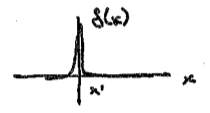
\includegraphics[width=.3\textwidth]{figures/lec10_.png}
    }}
  \ . 
\end{align}
Note that the source is \emph{zero} for everywhere. This means that everywhere to the left of $x=x'$ is described by a homogeneous equation,
\begin{align}
  \mathcal O_x G_<(x,x') = 0 \ .
\end{align}
Further, everything to the right of $x=x'$ is described by \emph{another} homogeneous equation,
\begin{align}
  \mathcal O_x G_>(x,x') = 0 \ .
\end{align}
These are different equations for \emph{different functions}: $G_<$ and $G_>$ are two different functions that obey homogeneous equations \emph{in their respective domains}. $G_<(x,x')$ is \emph{not} defined for $x>x'$. Usually solving homogeneous equations is easier\footnote{I wouldn't really know, but it seems to take less time on \emph{Mathematica} so there you go.}. 

The strategy then  is to solve for $G_<(x,x')$ and $G_>(x,x')$ as functions of $x$ and \emph{patch them together}: 
\begin{align}
  G(x,x') = 
  \begin{cases}
  G_<(x,x') & \text{ if } x<x'\\
  G_>(x,x') & \text{ if } x>x'
  \end{cases}\ .
\end{align}

Here $x'$ is just a spectator variable---we're keeping it fixed. For simplicity, you may even want to shift your coordinates so that $x'=0$. When we do this, we usually have a second order differential equation---some variant of the Laplacian because that's 99\% of what we do---so we need to have enough boundary conditions to fix our cofficients. Since we have two functions in a second order differential equation, we need \emph{four} boundary conditions. When we defined the Green's function problem, presumably we are considering functions over some interval $x,x'\in [a,b]$. This gives boundary conditions at $a$ and $b$, which may even be at $a=-\infty$ and $b=\infty$. The two additional boundaries are obtained at $x=x'$. These come from requiring the continuity of the solutions
\begin{align}
  G_<(x',x') = G_>(x',x')
\end{align}
and a `jump condition' between the first derivatives of the soltuion:
\begin{align}
  \lim_{\epsilon\to 0}\int_{x'-\epsilon}^{x'+\epsilon}dx \mathcal O_x G_(x,x') = 1 \ ,
\end{align}
where this comes from simply integrating the defining equation $\mathcal O_xG(x,x') = \delta(x-x')$ over a sliver around $x=x'$. Since $\mathcal O_x$ is assumed to be second order, the jump condition reduces to saying that the first derivatives of $G_<$ and $G_>$ are discontinuous at $x=x'$ by a certain amount. Applying these boundary conditions then gives a piece-wise solution for the Green's function.


\section{Where we're going}
\label{sec:ways:to:solve:G}

Our primary goal in this course is to find the Green's function $G(x,x')$ given a differential operator $\mathcal O$. There are three primary ways to do this:
\begin{enumerate}
\item \textbf{Eigenfunctions and completeness}, Section~\ref{sec:Greens:fuctions:by:completeness}. Assuming one knows the eigenfunctions of the differential operator, this gives a series solution for the Green's function. It is practically useful only when the series is convergent.

\item \textbf{Patching}, Section~\ref{sec:patching}. This method assume that one can solve the \emph{homogeneous} differential equation $\mathcal O_x G(x,x')=0$ and then produces a piece-wise solution to the \emph{inhomogeneous} differential equation that defines the Green's function, $\mathcal O_x G(x,x')=\delta(x-x')$. This is practically useful in one dimension where the boundary conditions where the pieces are connected are easy to define.

\item \textbf{Fourier transform and its cousins}. This will be the topic of the rest of our course. We convert the differential equation into an \emph{algebraic equation} in momentum space. Aspects of the causal structure of the system that are manifested in complex momentum space. Furthermore, one can use contour integrals to do the `hard work.'
\end{enumerate}

Recently I filled a hole in my undergraduate education and used a fourth method called the \emph{method of variations} to solve inhomogeneous differential equations. The method is sketched out in Appendix~\ref{app:method:of:variations}. We won't have anything further to say about that here, except that it turns out you can get a faculty job in theoretical particle physics without knowing how to use it.

\begin{example}
This problem is from Matthews \& Walker Section 9-4. Consider a unit string with frequency $k= \omega/c$ and Dirichlet boundary conditions at $x=0,1$; where we note that we are using units of `length of the string.' The differential operator describing standing waves is
\begin{align}
  \mathcal O_x = \frac{d^2}{dx^2} + k^2 \ .
 \end{align}
Let's solve this using eigenfunctions. We know the normalized eigenfunctions from Example~\ref{ex:summary:eigenfunction:fourier}:
\begin{align}
  f_n(x) &= \sqrt{2} \sin (n\pi x) 
  &
  \mathcal O_x f_n(x) 
  & = \left(-n^2\pi^2 + k^2\right)f_n(x) \equiv \lambda_n f_n(x) \ .
\end{align}
By the way, it should  have been \emph{obvious} that these are the eigenfunctions and eigenvalues, even though $\mathcal O_x$ is \emph{not} the same as $d^2/dx^2$. Using our completeness relation, the Green's function is
\begin{align}
  G(x,x') &= \sum_n \frac{f^*(x)f(x')}{\lambda_n}
  =
  2\sum_n\frac{\sin(n\pi x) \sin (n\pi x')}{k^2 - n^2\pi^2} \ .
\end{align}
Thus the solution to the system with some inhomogeneous source $s(x)$
\begin{align}
  \left[\frac{d^2}{dx^2} + k^2\right] f(x) &= s(x)
\end{align}
is simply
\begin{align}
  f(x) &= \int_0^1 dx' \, G(x,x') s(x') \ .
\end{align}
\end{example}

\begin{example}\label{ex:patching:eg}
Let's do the same example with the patching method. In this case we start with the equation (the analog of $A(A^{-1}) =\mathbbm{1}$):
\begin{align}
  \left[\frac{d^2}{dx^2} + k^2\right]G(x,x') &= \delta(x-x')
\end{align}
We now separate the domain into $x<x'$ and $x>x'$, with \emph{a priori} independent solutions $G_<(x,x')$ and $G_>(x,x')$:
\begin{center}
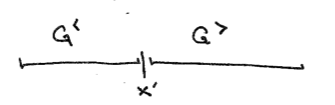
\includegraphics[width=.5\textwidth]{figures/lec11_GgGl.png}
\end{center}
Applying the Dirichlet boundary conditions at $x=0,1$ gives
\begin{align}
  G(x,x') &=
  \begin{cases}
  G_<(x,x') = a\sin(kx) & \text{ for } x < x'\\
  G_>(x,x') = b\sin\left(k(x-1)\right) & \text{ for } x > x'
  \end{cases} \ .
\end{align}
Make sure you understand why $G_>(x,x')$ has a factor of $(x-1)$ and not $x$; this is simply the boundary condition at $x=1$ without setting $b=0$.
The two coefficients $a$ and $b$ must be fixed by the matching at $x=x'$. 
To do this, integrate the second order differential equation over a sliver around $x'$:
\begin{align}
  \int_{x'-\varepsilon}^{x'+\varepsilon}
  \D{x} \, 
  \left[
   \frac{d^2}{dx^2} + k^2
  \right]
  G(x,x')
  &=
  \int_{x'-\varepsilon}^{x'+\varepsilon} dx\, \delta (x-x') \ .
  \label{eq:eg:jump:condition:integration:eg:1}
\end{align}
Note that the $k^2 G$ term in the integrand vanishes since it scales like $\varepsilon$. The integral of the second derivative is simple since it is simply the integral of a derivative, $\int dx\, d/dx(G') = \int d(G') = G'$ so that
\begin{align}
  \left.\frac{d}{dx}G\right|_{x'-\varepsilon}^{x'+\varepsilon}
  &=
  G'_>(x',x') - G'_<(x',x')
  =
   1 \ .
   \label{eq:eg:patching:jump:condition}
\end{align}
This is the jump condition of the first derivative. If we integrate the jump condition once more over a sliver between $x\pm\varepsilon$ gives the continuity condition:
\begin{align}
  G_<(x',x') &= G_>(x',x') \ .
\end{align}
If you are very attentive to details, you may be concerned about doing another integration since \eqref{eq:eg:patching:jump:condition} is simply an equality between numbers. If you are this attentive, I refer to the next example.
The jump and continuity conditions give
\begin{align}
  ka \cos(kx') + 1 &= kb \cos \left(k(x'-1)\right)
  \\
  a\sin(kx') &= b\sin \left(k(x'-1)\right) .
\end{align}
One can solve for the coefficients:
\begin{align}
  a&= \frac{\sin \left(k(x'-1)\right)}{k\sin k}
  &
  b&= \frac{\sin kx'}{k\sin k} \ .
\end{align}
Plugging this all in gives 
\begin{align}
  G(x,x') &=
  \frac{1}{k\sin k}
  \begin{cases}
  \sin kx \, \sin \left(k(x'-1)\right) &\text{ if }x < x'
  \\
  \sin kx' \, \sin \left(k(x-1)\right) &\text{ if }x > x' \ .
  \end{cases}
\end{align}
\end{example}
Observe that you find two \emph{different} expressions for $G$ by these methods. Please confirm---perhaps numerically---that these indeed represent the same function $G(x,x')$. 

\begin{example}%{ex:patching:second:integration}
In the previous example, we integrated the Green's function equation `twice' to get two boundary conditions at $x=x'$. You may be concerned that after doing the first definite integral, we just have a relation between numbers. That is to say, we can no longer `integrate a total derivative' $\int dx\; \partial_x f(x) = f(x)$ because the integrand is not a total derivative, it is just a number. 

It may be helpful to think about this as follows. The first definite integral of the Green's function equation gives the jump condition, \eqref{eq:eg:patching:jump:condition}. For the second integral, we may take
\begin{align}
  \int_{-\varepsilon'}^{\varepsilon'}
  dy \,
  \int_{x'-\varepsilon}^{x'+\varepsilon+y}
  \D{x} \, 
  \left[
   \frac{d^2}{dx^2} + k^2
  \right]
  G(x,x')
  &=
  \int_{-\varepsilon'}^{\varepsilon'}
  dy \,
  \int_{x'-\varepsilon}^{x'+\varepsilon+y}
  \D{x} \, 
  \delta (x-x') 
  \ .
\end{align}
One can compare to \eqref{eq:eg:jump:condition:integration:eg:1}. You should be happy that the right-hand side integrates to zero upon $\varepsilon\, , \, \varepsilon' \to 0$; it is two integrations over an infinitesimal slice with only one $\delta$-function to support it. Following through gives:
\begin{align}
  \int_{-\varepsilon'}^{\varepsilon'}
  dy \,
  \int_{x'-\varepsilon}^{x'+(\varepsilon+y)}
  \D{x} \, 
  \frac{d}{dx}
  \left[
   \frac{d}{dx}
   G(x,x')
  \right]
  &=
  \int_{-\varepsilon'}^{\varepsilon'}
  dy \,
  \left[
   G'(x'+y+\varepsilon,x')
   -
   G'(x'-\varepsilon, x')
  \right] \ .
\end{align}
$G'(x'-\varepsilon, x')$ is simply a constant. Its integral vanishes when we take the limit $\varepsilon\, ,\, \varepsilon'\to 0$. For the first term, we may strategically take $\varepsilon\to 0$  (or otherwise $\varepsilon < \varepsilon'$) so that we now have
\begin{align}
  \int_{-\varepsilon'}^{\varepsilon'}
  dy \,
  \frac{d}{dy}
  \left[
   G(x'+y+\varepsilon,x')
   \right] \ .
\end{align}
Note the subtle sleight of hand: $G'(\cdots, x')$ means ``take the derivative of $G$ with respect to the first argument.'' The variable in the first argument is $y$, so we have written it out explicitly as $d/dy$ so that the $dy$ integral is over a total derivative. This now straightforwardly gives, 
\begin{align}
  G(x'+\varepsilon+\varepsilon', x') 
  -
  G(x'+\varepsilon-\varepsilon', x') 
  = 0 \ ,
\end{align}
which is simply the continuity condition \eqref{eq:eg:patching:jump:condition} once we choose $\varepsilon' > \varepsilon$ with both going to zero.
\end{example}

\begin{exercise}
This example is from Butkov, chapter 12.1. Consider a taut string of length $L$ under the load of a weirdly-shaped rock:
\begin{center}
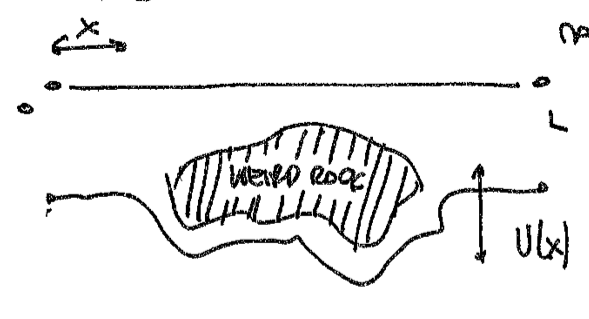
\includegraphics[width=.5\textwidth]{figures/lec12_eg.png}
\end{center}
The force equation for the vertical displacement of the string, $u(x)$, is
\begin{align}
  T u''(x) = F(x),
\end{align}
where $T$ is the tension and $F(x)$ is the force-per-unit-length. One may write this more simply as $u''(x) = f(x) = F(x)/T$. Show that the Green's function may be written as a piecewise function
\begin{align}
  G(x,x') &=
  \begin{cases}
  \left(\frac{x'-L}{L}\right)x  & \text{ if } x<x'
  \\
  \left(\frac{x-L}{L}\right)x' & \text{ if } x>x' 
  \end{cases}\ .
\end{align}
Suppose you replace the weird rock by a square paper weight of size $x < L$ in the middle of the string. Sketch what the paper weight on the string looks like.
\end{exercise}


\section{Example: Stability Analysis (Extra topic)}

% From Numerical Recipes, Ch 20 on PDEs
Suppose we want to solve a partial differential equation numerically.\footnote{This section draws from \emph{Numerical Recipes} by Press et al. The book is a classic but is sometimes overlooked for silly reasons: perhaps it is too old to be relevant for modern computing? Perhaps it is too computational for theorists? Wrong.} We discretize space and time into bins of size $\Delta x$ and $\Delta t$:
\begin{align}
  x_a &= x_0 + a\Delta x & t_n = t_0 + n\Delta t \ .
\end{align}
Suppose we have a simple wave equation for a quantity $u(x,t)$:
\begin{align}
  \partial_t u(x,t)= - v\partial_x u(x,t) \ .
\end{align}
In our discretization, let $u^n_a\equiv u(x_a,t_n)$.
If we choose a space-symmetric spatial derivative, we may write the discretized wave equation as:
\begin{align}
\frac{u^{n+1}_a - u^{n}_a}{\Delta t}
=
-v\left(\frac{u^n_{a+1}-u^n_{a-1}}{2\Delta x}\right) \ .
\end{align}
Suppose we have \emph{initial data} about the configuration, $u(t_0, x)$ for all $x$. The discretization gives a way to numerically calculate the configuration over all $x$ at the next slice in $t$:
\begin{align}
  u_a^{n+1} = u^n_a 
  + \Delta t
  \left[-v\left(\frac{u^n_{a+1}-u^n_{a-1}}{2\Delta x}\right)\right] \ .
  \label{eq:FTCS}
\end{align}
This is called the Euler algorithm, or more precisely a \emph{forward time centered space} representation. This is clearly a numerical approximation to a continuous equation. A good question is: how good of an approximation is it?

There's a method call the Von Neumann stability analysis that uses Fourier series to answer this question. This analysis was invented by Clark and Nicolson rather than the physicist and computer scientist John von Neumann after whom it is named.\footnote{This is Stigler's law of eponymy. Stigler himself explains that he was not the first to present the idea.} The idea is to write $u^n_a$ as a Fourier series over plane waves with momentum (wave number) $k$:
\begin{align}
  u^n_a \sim  e^{ika\Delta x} \ .
\end{align}
Plugging this into \eqref{eq:FTCS} gives
\begin{align}
  u^{n+1}_a = 
  \left[1 - i v\frac{\Delta t}{\Delta x}\sin k\Delta x\right]u^n_a \ ,
\end{align}
where we identify the bracketed term as a $k$-dependent prefactor $c(k)$:
\begin{align}
   c(k) = 1 - i v\frac{\Delta t}{\Delta x}\sin k\Delta x \ .
\end{align}
The time evolution of a given $k$ mode is simply a power of $c(k)$:
\begin{align}
  u^{n}_a &= c(k)^n e^{ika\Delta x} \ .
\end{align}
Our expression for $c(k)$ is a complex number with modulus strictly greater than 1 for all $k$. That means that the prefactor of \emph{any} mode diverges. The numerical integration scheme is intrinsically unstable. This is often expressed as the statement: never use Euler forward differencing when numerically solving a differential equation.

Our analysis was strictly for the wave equation: a first order partial differential equation with constant coefficients. A more sophisticated partial differential equation has coefficients that may depend on space and time. The Von Neumann analysis is valid as long as the coefficients vary slowly relative to our discretization.

\begin{exercise}
There are simple tweaks to our integration method that can cure the forward differencing instability. One method is called the Lax method. The proposal is to write the time derivative in a funny way:
\begin{align}
  \partial_t u(t_n, x_a) \to
  \frac{
    u^{n+1}_a 
    - \frac{1}{2}\left(u^n_{a-1}+u^n_{a+1}\right)
    }{ \Delta t } \ .
\end{align}
Show that this modifies the Von Neumann analysis to give a coefficient
\begin{align}
  c(k) = \cos k\Delta x - i v\frac{\Delta t}{\Delta x}\sin k\Delta x \ ,
\end{align}
so that the stability condition is
\begin{align}
\frac{\Delta t}{\Delta x} \leq |v| \ .
\end{align}
This condition is called the Courant condition and is fairly generic for numerical solutions to first-order differential equations.
\end{exercise}


\begin{subappendices}

\section{Method of Variations}
\label{app:method:of:variations}

The method of variations is a way to solve inhomogeneous differential equations starting from a basis of solutions to the homogeneous differential equation. We specialize to the case of second-order differential operators, though the technique is valid for higher-order operators.

\subsection{First order equation for coefficients}

Consider the second-order inhomogeneous linear differential equation
\begin{align}
	\mathcal Of(x) &= a_2(x)f''(x) + a_1(x) f'(x) + a_0(x) = g(x) \ .
\end{align}
One can determine the solution to this equation from varying with respect to the solutions to the homogeneous differential equation, $u(x)$ and $v(x)$. Write the solution to the inhomogeneous equation as
\begin{align}
	f(x) &= c(x)u(x) + d(x)v(x)
\end{align}
Make the ansatz that
\begin{align}
	c'(x) u(x) + d'(x) v(x) = 0 \ .
	\label{eq:method:of:variations:ansatz}
\end{align}
Then the inhomogeneous differential equation reduces to
\begin{align}
	\mathcal Of &= a_2(x)\left(c'(x) u'(x) + d'(x) v'(x)\right) =g(x) \ .
\end{align}
This gives expressions for $c'$ and $d'$:
\begin{align}
	c'(x) &= \frac{-v(x)g(x)/a_2(x)}{u(x) v'(x) - u'(x) v(x)}
	&
	d'(x) &= \frac{u(x)g(x)/a_2(x)}{u(x) v'(x) - u'(x) u(x)} \ ,
	\label{eq:method:of:variations:first:order}
\end{align}
where one may recognize the denominators to be the Wronksian, $W = uv' - u'v$. For simplicity, write $\tilde g(x) \equiv g(x)/a_2(x)$.
% Integrating these equations then gives the solution to the inhomogeneous equation. 

\subsection{Integrating and boundary conditions}

Suppose that the inhomogeneous differential equation has boundary conditions at $x_1$ and $x_2$ given by differential operators $\mathcal B_{1,2}$:
\begin{align}
	\mathcal B_1 f(x) &= \alpha_1 f'(x_1) + \beta_1 f(x_1) &= 0
	\\
	\mathcal B_2 f(x) &= \alpha_2 f'(x_2) + \beta_2 f(x_2) &= 0 \ .
\end{align}
These boundary conditions are, in general, first order for a second order inhomogeneous differential equation. For example, these may come from integrating a second-order equation of motion by parts, leaving a first-order operator on either boundary.
%
The ansatz \eqref{eq:method:of:variations:ansatz} simplifies these boundary conditions:
\begin{align}
	\mathcal B_i f(x) &= 
	c(x_i) \mathcal B_i u (x) 
	+
	d(x_i) \mathcal B_i v (x) 
	= 0 
	\ .
	\label{eq:method:of:variations:BC}
\end{align}
For simplicity, let us write $(\mathcal B_i u) = \alpha_i u'(x_i) + \beta_i f(x_i)$ as a constant that depends on $u$ and $u'$ evaluated at the boundary $x_i$. We define $(\mathcal B_i v)$ similarly. 

Integrate the first-order differential equations for the coefficients \eqref{eq:method:of:variations:first:order} using these boundary conditions. The simplest approach is to integrate a convenient linear combinations:
\begin{align}
	\mathcal{I}_1 = 
	\int_{x_1}^x
	\D{y}\, c'(y)(\mathcal B_1 u) + d'(y) (\mathcal B_1 v)
	&= c(x) (\mathcal B_1 u) + d(x) (\mathcal B_1 v) \ ,
	\label{eq:method:of:variations:int:1}
\end{align}
where the lower limit vanishes because $(\mathcal B_i f) \equiv 0$. Similarly, one finds
\begin{align}
	\mathcal{I}_2 = 
	\int_{x}^{x_2}
	\D{y}\, c'(y)(\mathcal B_2 u) + d'(y) (\mathcal B_2 v)
	&= -c(x) (\mathcal B_2 u) - d(x) (\mathcal B_2 v) \ .
	\label{eq:method:of:variations:int:2}
\end{align}
The integrals in \eqref{eq:method:of:variations:int:1} and \eqref{eq:method:of:variations:int:2} are equivalently expressed using the expressions for $c'(x)$ and $d'(x)$ in \eqref{eq:method:of:variations:first:order}:
% \begin{align}
% 	\int_{x_1}^x
% 	\D{y}\, c'(y)(\mathcal B_1 u) + d'(y) (\mathcal B_1 v)
% 	&= 
% 	\int_{x_1}^x dy \,
% 	\frac{-v(y)
% 	% g(x)/a_2(x)
% 	\tilde g(y)
% 	}{W(y)}
% 	(\mathcal B_1 u)
% 	+ 
% 	\frac{u(y)
% 	%g(x)/a_2(x)
% 	\tilde g(y)
% 	}{W(y)}
% 	(\mathcal B_1 v) 
% 	\\
% 	\int_{x}^{x_2}
% 	\D{y}\, c'(y)(\mathcal B_2 u) + d'(y) (\mathcal B_2 v)
% 	&=
% 	\int_{x}^{x_2}
% 	\D{y}\, \frac{-v(y)
% 	%g(x)/a_2(x)
% 	\tilde g(y)
% 	}{W(y)} 
% 	(\mathcal B_2 u) 
% 	+ \frac{u(y)
% 	%g(x)/a_2(x)
% 	\tilde g(y)
% 	}{W(y)} 
% 	(\mathcal B_2 v)
% 	\ .
% \end{align}
\begin{align}
	\mathcal{I}_1 
	%= 
	% \int_{x_1}^x
	% \D{y}\, c'(y)(\mathcal B_1 u) + d'(y) (\mathcal B_1 v)
	&= 
	\int_{x_1}^x dy \,
	\left[
	- (\mathcal B_1 u) v(y)
	+ (\mathcal B_1 v) u(y)
	\right]
	\frac{
	\tilde g(y)
	}{W(y)}	
	\\
	\mathcal{I}_2 
	% = 
	% \int_{x}^{x_2}
	% \D{y}\, c'(y)(\mathcal B_2 u) + d'(y) (\mathcal B_2 v)
	&=
	\int_{x}^{x_2}
	\D{y}\, 
	\left[  - (\mathcal B_2 u) v(y) 
			+ (\mathcal B_2 v) u(y)
	\right]
	\frac{
	\tilde g(y)
	}{W(y)} 
	\ .
\end{align}
Combining this with the right-hand sides of \eqref{eq:method:of:variations:int:1} and \eqref{eq:method:of:variations:int:2} then gives the desired integral solutions for the coefficient functions:
\begin{align}
	\left[ \left(\mathcal B_1 u\right)\left(\mathcal B_2 v\right) - \left(\mathcal B_2 u\right)\left(\mathcal B_1 v\right)  \right]
	c(x)
	&= 
	% \phantom{+}
	\left(\mathcal B_2 v\right)
	\mathcal{I}_1 
	% \int_{x_1}^x dy \,
	% \left[
	% - (\mathcal B_1 u) v(y)
	% + (\mathcal B_1 v) u(y)
	% \right]
	% \frac{
	% \tilde g(y)
	% }{W(y)}	
	% \\
	% &\phantom{=}
	+
	\left(\mathcal B_1 v\right)
	% \int_{x}^{x_2}
	% \D{y}\, 
	% \left[  - (\mathcal B_2 u) v(y) 
	% 		+ (\mathcal B_2 v) u(y)
	% \right]
	% \frac{
	% \tilde g(y)
	% }{W(y)} 
	\mathcal{I}_2 
	\\
	\left[ 
		\left(\mathcal B_2 u\right)\left(\mathcal B_1 v\right) 
		- 
		\left(\mathcal B_1 u\right)\left(\mathcal B_2 v\right)  
	\right]
	d(x)
	&= 
	\left(\mathcal B_2 u\right)
	\mathcal{I}_1 
	+ 
	\left(\mathcal B_1 u\right)
	\mathcal{I}_2 
	\ .
\end{align}
% Similarly for the $d(x)$ coefficient:
% \begin{align}
% 	\left[ 
% 		\left(\mathcal B_2 u\right)\left(\mathcal B_1 v\right) 
% 		- 
% 		\left(\mathcal B_1 u\right)\left(\mathcal B_2 v\right)  
% 	\right]
% 	d(x)
% 	&= 
% 	\phantom{+}
% 	\left(\mathcal B_2 u\right)
% 	\int_{x_1}^x dy \,
% 	\left[
% 	- (\mathcal B_1 u) v(y)
% 	+ (\mathcal B_1 v) u(y)
% 	\right]
% 	\frac{
% 	\tilde g(y)
% 	}{W(y)}	
% 	\\
% 	&\phantom{=}+
% 	\left(\mathcal B_1 u\right)
% 	\int_{x}^{x_2}
% 	\D{y}\, 
% 	\left[  - (\mathcal B_2 u) v(y) 
% 			+ (\mathcal B_2 v) u(y)
% 	\right]
% 	\frac{
% 	\tilde g(y)
% 	}{W(y)} 
% 	\ .
% \end{align}
Define the left-hand side prefactors:
\begin{align}
	(\text{den}.) &\equiv
	\left(\mathcal B_1 u\right)\left(\mathcal B_2 v\right) - \left(\mathcal B_2 u\right)\left(\mathcal B_1 v\right)  \ ,
\end{align}
so that we have 
\begin{align}
	f(x) &= 
	\frac{\left(\mathcal B_2 v\right)
		\mathcal{I}_1 
		+
		\left(\mathcal B_1 v\right)
		\mathcal{I}_2}{(\text{den.})}
	u(x)
	-
	\frac{\left(\mathcal B_2 u\right)
		\mathcal{I}_1 
		+
		\left(\mathcal B_1 u\right)
		\mathcal{I}_2}{(\text{den.})}
	v(x)
\end{align}
\begin{wide}
Collecting the terms by the integration range gives:
\begin{align}
	(\text{den.})f(x)&=
	\int_{x_1}^x dy \frac{\tilde g(y)}{W(y)}
	\left[
		-(\mathcal B_1u)(\mathcal B_2u) v(x)v(y)
		+(\mathcal B_1v)(\mathcal B_2v) u(x)u(y)
		\right.
	\\
	&\phantom{=\int_{x_1}^x D{y} \frac{\tilde g(y)}{W(y)}[}
		\left.
		-(\mathcal B_1u)(\mathcal B_2v) u(x)v(y)
		+(\mathcal B_1v)(\mathcal B_2u) v(x)u(y)
	\right] + \cdots
	\\
	&=
	\int_{x_1}^x \D{y} \frac{\tilde g(y)}{W(y)}
	\left[
		(\mathcal B_1u)v(y) - (\mathcal B_1v)u(y)
	\right] 
	\left[
		(\mathcal B_2u)v(x) - (\mathcal B_2v)u(x)
	\right] + \cdots \ .
\end{align}
The $\cdots$ represent the $\mathcal I_2$ terms. Performing the same grouping for the $\mathcal I_2$ terms then gives:
\begin{align}
	(\text{den.})f(x)&=
	\int_{x_1}^x \D{y} \frac{\tilde g(y)}{W(y)}
	\left[
		(\mathcal B_1u)v(y) - (\mathcal B_1v)u(y)
	\right] 
	\left[
		(\mathcal B_2u)v(x) - (\mathcal B_2v)u(x)
	\right] + \\
	&\phantom{=}
	\int_{x}^{x_2} \D{y} \frac{\tilde g(y)}{W(y)}
	\left[
		(\mathcal B_1v)u(x) - (\mathcal B_1u)v(x)
	\right] 
	\left[
		(\mathcal B_2v)u(y) - (\mathcal B_2u)v(y)
	\right] \ .
\end{align}
These two terms can be combined rather nicely:
\begin{align}
	f(x) &=
	\frac{1}{(\text{den.})}
	\int_{x_1}^{x_2} \D{y} \,
	\frac{\tilde g(y)}{W(y)}
	\left[
		(\mathcal B_1u)v(x_<) - (\mathcal B_1v)u(x_<)
	\right] 
	\left[
		(\mathcal B_2u)v(x_>) - (\mathcal B_2v)u(x_>)
	\right]
\end{align}
where we introduce the convenient notation that
\begin{align}
	x_< &= \min(x,y)
	&
	x_> &= \max(x,y) \ .
\end{align}
\end{wide}

\end{subappendices}